% This file was created with tikzplotlib v0.10.1.
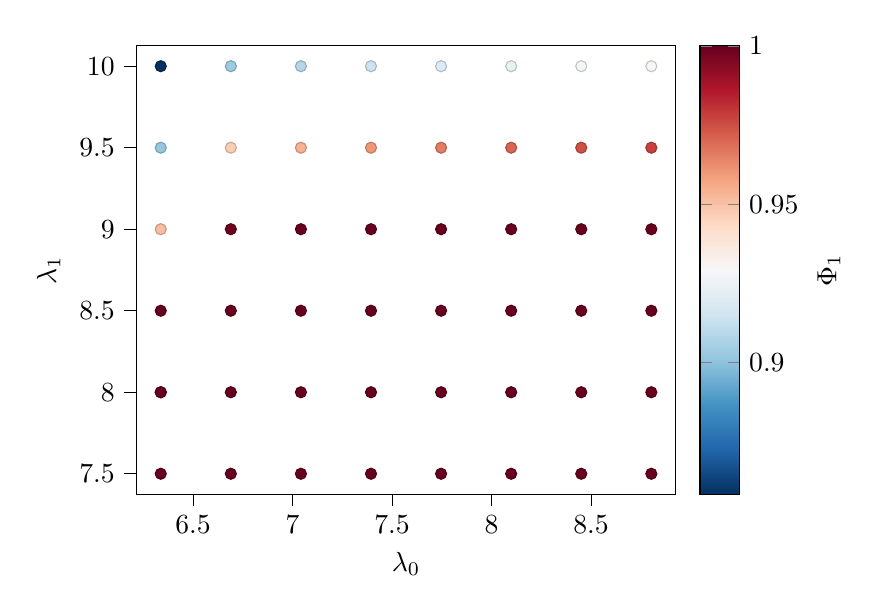
\begin{tikzpicture}

\definecolor{darkgray176}{RGB}{176,176,176}

\begin{axis}[
colorbar,
colorbar style={ylabel={$\Phi_{1}$}},
colormap={mymap}{[1pt]
  rgb(0pt)=(0.0196078431372549,0.188235294117647,0.380392156862745);
  rgb(1pt)=(0.129411764705882,0.4,0.674509803921569);
  rgb(2pt)=(0.262745098039216,0.576470588235294,0.764705882352941);
  rgb(3pt)=(0.572549019607843,0.772549019607843,0.870588235294118);
  rgb(4pt)=(0.819607843137255,0.898039215686275,0.941176470588235);
  rgb(5pt)=(0.968627450980392,0.968627450980392,0.968627450980392);
  rgb(6pt)=(0.992156862745098,0.858823529411765,0.780392156862745);
  rgb(7pt)=(0.956862745098039,0.647058823529412,0.509803921568627);
  rgb(8pt)=(0.83921568627451,0.376470588235294,0.301960784313725);
  rgb(9pt)=(0.698039215686274,0.0941176470588235,0.168627450980392);
  rgb(10pt)=(0.403921568627451,0,0.12156862745098)
},
point meta max=1,
point meta min=0.858471498267994,
tick align=outside,
tick pos=left,
x grid style={darkgray176},
xlabel={\(\displaystyle \lambda_{0}\)},
xmin=6.2147887314, xmax=8.9260563366,
xtick style={color=black},
y grid style={darkgray176},
ylabel={\(\displaystyle \lambda_{1}\)},
ymin=7.375, ymax=10.125,
ytick style={color=black}
]
\addplot [
  colormap={mymap}{[1pt]
  rgb(0pt)=(0.0196078431372549,0.188235294117647,0.380392156862745);
  rgb(1pt)=(0.129411764705882,0.4,0.674509803921569);
  rgb(2pt)=(0.262745098039216,0.576470588235294,0.764705882352941);
  rgb(3pt)=(0.572549019607843,0.772549019607843,0.870588235294118);
  rgb(4pt)=(0.819607843137255,0.898039215686275,0.941176470588235);
  rgb(5pt)=(0.968627450980392,0.968627450980392,0.968627450980392);
  rgb(6pt)=(0.992156862745098,0.858823529411765,0.780392156862745);
  rgb(7pt)=(0.956862745098039,0.647058823529412,0.509803921568627);
  rgb(8pt)=(0.83921568627451,0.376470588235294,0.301960784313725);
  rgb(9pt)=(0.698039215686274,0.0941176470588235,0.168627450980392);
  rgb(10pt)=(0.403921568627451,0,0.12156862745098)
},
  only marks,
  scatter,
  scatter src=explicit
]
table [x=x, y=y, meta=colordata]{%
x  y  colordata
6.338028168 7.5 1.0
6.338028168 8 1.0
6.338028168 8 1.0
6.338028168 8.5 1.0
6.338028168 9 0.9512339390680409
6.338028168 9.5 0.9019771621788216
6.690140844 7.5 1.0
6.690140844 8 1.0
6.690140844 8.5 1.0
6.690140844 9 0.998870639678856
6.690140844 9.5 0.947152960358294
6.690140844 10 0.9030855198179061
7.04225352 7.5 1.0
7.04225352 8 1.0
7.04225352 8.5 1.0
7.04225352 9 0.9999589989162081
7.04225352 9.5 0.9544670743738127
7.04225352 10 0.9086694068785041
7.394366196 7.5 1.0
7.394366196 8 1.0
7.394366196 8.5 1.0
7.394366196 9 1.0
7.394366196 9.5 0.9604896315732091
7.394366196 10 0.9144103572407271
7.746478872 7.5 1.0
7.746478872 8 1.0
7.746478872 8.5 1.0
7.746478872 9 1.0
7.746478872 9.5 0.9660089342710694
7.746478872 10 0.9196919623398475
8.098591548 7.5 1.0
8.098591548 8 1.0
8.098591548 8.5 1.0
8.450704224 7.5 1.0
8.450704224 8 1.0
8.450704224 8.5 1.0
8.8028169 8 1.0
8.8028169 8.5 1.0
8.098591548 9 1.0
8.098591548 9.5 0.9707153102943908
8.098591548 10 0.9237716836487669
8.450704224 9 1.0
8.450704224 9.5 0.9747973720349585
8.450704224 10 0.927895490861111
8.8028169 9 1.0
8.8028169 9.5 0.9777818380506861
8.8028169 10 0.9304941786452393
6.338028168 10 0.858471498267994
8.8028169 7.5 1.0
};
\end{axis}

\end{tikzpicture}
